% ------------------------------------------------------------------------
% file `3_thales_similitudes-transferer-6-exercise-body.tex'
%   in folder `xsim/'
%
%     exercise of type `transferer' with id `6'
%
% generated by the `transferer' environment of the
%   `xsim' package v0.21 (2022/02/12)
% from source `3_thales_similitudes' on 2023/06/09 on line 220
% ------------------------------------------------------------------------
    D'après le code de la route, les feux de croisement d'une voiture permettent d'éclairer efficacement la route, la nuit par temps clair, sur une distance de \SI{30}{m}.

    Afin de contrôler régulièrement la portée des feux de sa voiture, Jacques veut tracer un repère sur le mur au fond de son garage.

    La figure n'est pas à l'échelle.

    \begin{center}
        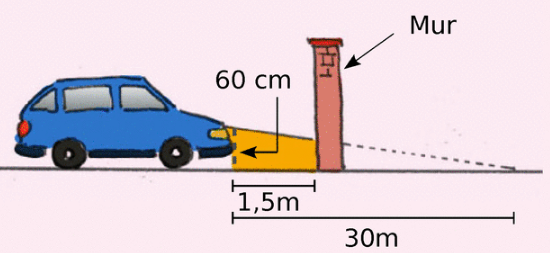
\includegraphics[width=.5\linewidth]{img/C3_voiture.png}
    \end{center}

    Les feux de croisement sont à \SI{60}{cm} du sol.

    À quelle hauteur doit-il placer le repère sur son mur pour pouvoir régler correctement ses phares ?
